\documentclass[a4paper, 15pt]{scrartcl}

\usepackage[utf8]{inputenc}
\usepackage[ngerman]{babel}
\usepackage[T1]{fontenc}
\usepackage{fancyhdr}
\usepackage{tikz}
\usepackage{graphicx}

\usetikzlibrary{automata, positioning}

\pagestyle{fancy}
\pagenumbering{gobble}

\title{SZS Blatt 1}
\author{
	Christian Baumann 3164561, st142624@stud.uni-stuttgart.de \\ 
	Ellen Hafner 3253401, st151037@stud.uni-stuttgart.de \\ 
	Marvin Knodel 3229587, st149003@stud.uni-stuttgart.de\\ 
	Lion Wagner 3231355, st148345@stud.uni-stuttgart.de}
\date{02.11.2018}

\lhead{Christian Baumann\\ Ellen Hafner\\ Marvin Knodel\\ Lion Wagner}
\rhead{3164561\\ 3253401\\ 3229587 \\ 3231355}

\begin{document}
	\maketitle
	\newpage
		\mbox{}
		\section*{Aufgabe 1}
		---
	\newpage
	
		\section*{Aufgabe 2}
			\subsection*{a)}
				\subsubsection*{Resilience}
					\textbf{Definitionen}
					\begin{enumerate}
						\item \grqq[...] Fähigkeit von technischen Systemen, bei Störung bzw. Teil-Ausfällen nicht vollständig zu versagen, sondern wesentliche Systemdienstleistungen aufrechtzuerhalten.\grqq \\
						(https://de.wikipedia.org/wiki/Resilienz\_(Ingenieurwissenschaften))
						
						\item \grqq an ability to recover from or adjust easily to misfortune or change\grqq\\ (https://www.merriam-webster.com/dictionary/resilience)
					\end{enumerate}
				
					\textbf{Beispiele}
					\begin{enumerate}
						\item Bei einem Stromausfall des SSB Netzes fahren keine Bahnen mehr dafür noch alle Busse. (zu Def. 1)
					
						\item Stärkung des Immunsystems nach einer Krankheit (z.B. Windpocken) \\(zu Def. 2)
					\end{enumerate}
				
				
				\subsubsection*{Survivability}
					\textbf{Definitionen}
					\begin{enumerate}
						\item \grqq[...] is the ability to remain alive or continue to exist.\grqq \\
						(https://en.wikipedia.org/wiki/Survivability)
					
						\item \grqq Capability of a system [...] to withstand a disaster or hastile environment, without significant impairment of its normal operations\grqq\\ (http://www.businessdictionary.com/definition/survivability.html)
					\end{enumerate}
				
					\textbf{Beispiele}
					\begin{enumerate}
						\item System stürzt über gesamte Betriebsdauer nicht ab. (zu Def. 1)
					
						\item Wüstenpflanzen überleben lange Dürreperioden. \\(zu Def. 2)
					\end{enumerate}
				
	\newpage
				\subsubsection*{Robustness}
					\textbf{Definitionen}
					\begin{enumerate}
						\item \grqq[...] is the property of being strong and healthy in constitution.\grqq \\
						(https://en.wikipedia.org/wiki/Robustness)
)
		
						\item \grqq[...] ability of a computer system to cope with errors during execution.\grqq\\ (https://www.thefreedictionary.com/robustness)
					\end{enumerate}
	
					\textbf{Beispiele}
					\begin{enumerate}
						\item Gesunder fitter Mensch. (zu Def. 1)
		
						\item Entwicklungsumgebung findet zu dem Projekt keine .exe aber anstatt abzustürzen erzeugt sie eine .exe Datei. \\(zu Def. 2)
					\end{enumerate}
	
	
					\subsubsection*{Complexity}
					\textbf{Definitionen}
					\begin{enumerate}
						\item \grqq[...] behavior of a system or model whose components interact in multiple ways and follow local rules.\grqq \\
						(https://en.wikipedia.org/wiki/Complexity)
		
						\item \grqq[...] state of having many different parts connected or related to each other in a complicated way\grqq\\ (https://www.collinsdictionary.com/dictionary/english/complexity)
					\end{enumerate}
	
					\textbf{Beispiele}
					\begin{enumerate}
						\item Komponenten eines Neuronale Netzes interagieren auf verschiedene Weise miteinander. (zu Def. 1)
		
						\item Quantencomputer sind sehr kompliziert aufgebaut. \\(zu Def. 2)
					\end{enumerate}
	
	\newpage
	
			\subsection*{b)}
				\subsubsection*{Elasticity}
					\textbf{Definitionen}
					\begin{enumerate}
						\item \grqq[...] is a measure of a variable's sensitivity ro a change in another variable.\grqq \\
						(https://www.investopedia.com/terms/e/elasticity.asp)
		
						\item \grqq [...] ability to resist or overcome depresion\grqq\\ (https://www.dictionary.com/browse/elasticity)
					\end{enumerate}
	
					\textbf{Beispiele}
					\begin{enumerate}
						\item Das Durchschnittsalter in einer Region steigt, wenn sich in dieser Region die medizinische Versorgung verbessert. (zu Def. 1)
		
						\item Depressive Menschen die ihre Depressionen überwinden.\\(zu Def. 2)
					\end{enumerate}
	
	
				\subsubsection*{Scalability}
					\textbf{Definitionen}
					\begin{enumerate}
						\item \grqq[...] Fähigkeit eines Systems, Netzwerks zur Größenveränderung.\grqq \\(https://en.wikipedia.org/wiki/Scalability)
		
						\item \grqq the ability of a business or system to grow larger.\grqq\\ (https://dictionary.cambridge.org/dictionary/english/scalability)
					\end{enumerate}
	
					\textbf{Beispiele}
					\begin{enumerate}
						\item Gameserver nachdem bei dem betroffenen Spiel die User Anzahl von wenigen auf sehr viele ansteigt aber die Server damit kein Problem haben. (zu Def. 1)
		
						\item Ein Unternehmen expandiert in ein neues Gebiet. \\(zu Def. 2)
					\end{enumerate}
	
	\newpage
				\subsubsection*{Efficiency}
					\textbf{Definitionen}
					\begin{enumerate}
						\item \grqq accomplishment of or ability to accomplish a job with a minimum expenditure of time and effort.\grqq(https://www.dictionary.com/browse/efficiency)
		
						\item \grqq The ratio of the useful work performed by a macchine or in a process to the total energy expanded or heat taken in.\grqq\\ (https://en.oxforddictionaries.com/definition/efficiency)
					\end{enumerate}
	
					\textbf{Beispiele}
					\begin{enumerate}
						\item Ich habe die Aufgabe schnell und mit wenig Aufwand gelöst.(zu Def. 1)
		
						\item LEDs erzeugen effizienter Licht als Glühbirnen.(zu Def. 2)
					\end{enumerate}
	
	
				\subsubsection*{Performability}
					\textbf{Definitionen}
					\begin{enumerate}
						\item \grqq The ability to perform,\grqq \\ (https://www.doc.ic.ac.uk/~nd/surprise\_95/journal/vol4/eaj2/report.html)
		
						\item \grqq A measurement of how well a system performs over a period of time, regardless of the presence of faults\grqq\\ (https://www.wordhippo.com/what-is/the-meaning-of-the-word/performability.\\html)
					\end{enumerate}
	
					\textbf{Beispiele}
					\begin{enumerate}
						\item Ein Computer ist dazu fähig verschiedene Programme auszuführen.\\(zu Def. 1)
		
						\item Angestellte sind von 10-bis 12 Uhr leistungsfähiger als von 13 bis 16 Uhr. \\(zu Def. 2)
					\end{enumerate}

		\newpage
	\section*{Aufgabe 3}
	\graphicspath{{D:/GoogleDrive/UNI/SZS/Blatt1/3/}{D:/GoogleDrive/UNI/SZS/Blatt1/4/}}

\subsection*{b)}

\begin{minipage}[h]{0.5\textwidth}
	\centering
	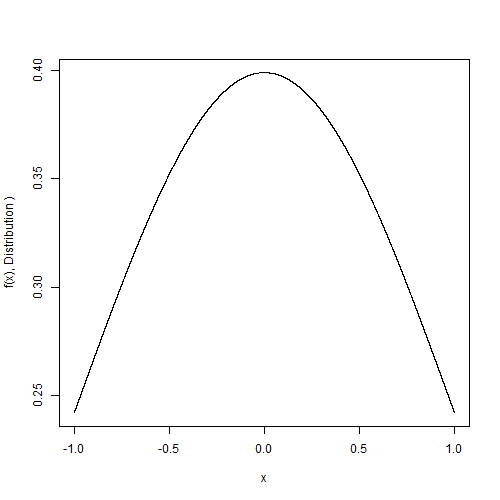
\includegraphics[width=0.8\textwidth]{bDistribution.png} 	
\end{minipage}\begin{minipage}[h]{0.5\textwidth}
	\centering
	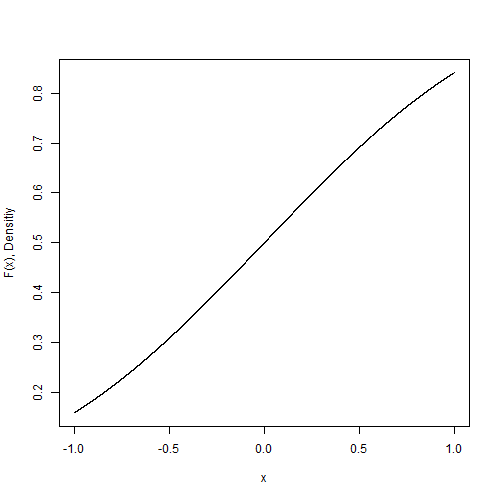
\includegraphics[width=0.8\textwidth]{bDensity.png}
\end{minipage}

\subsection*{c)}

\begin{minipage}[h]{0.5\textwidth}
	\centering
	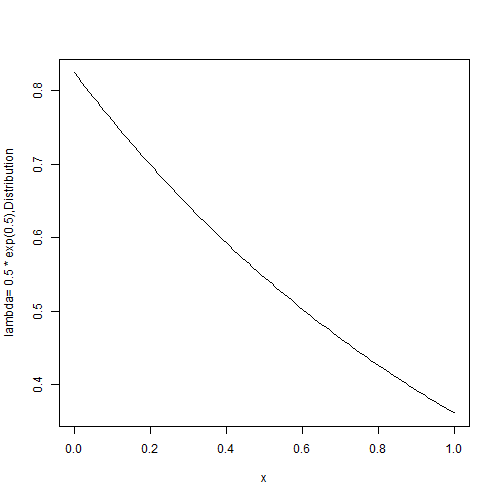
\includegraphics[width=0.8\textwidth]{c1.png} 
	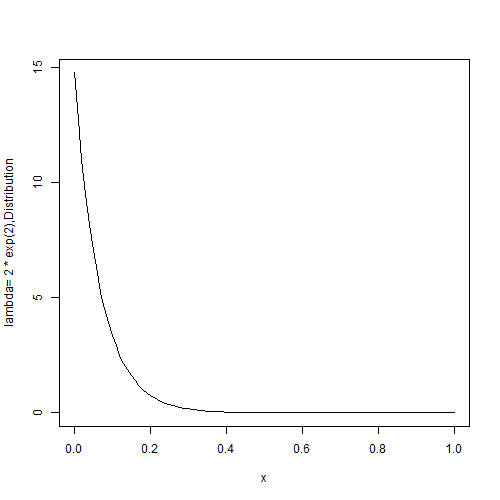
\includegraphics[width=0.8\textwidth]{c3.png} 		
\end{minipage}\begin{minipage}[h]{0.5\textwidth}
	\centering
	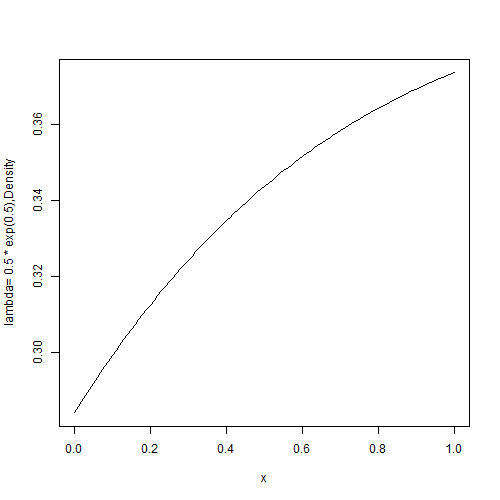
\includegraphics[width=0.8\textwidth]{c2.png}
	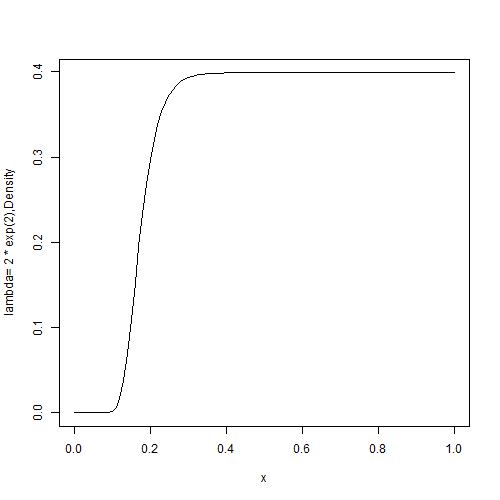
\includegraphics[width=0.8\textwidth]{c4.png} 	
\end{minipage}

\subsection*{d)}
\begin{minipage}[h]{0.5\textwidth}
	\centering
	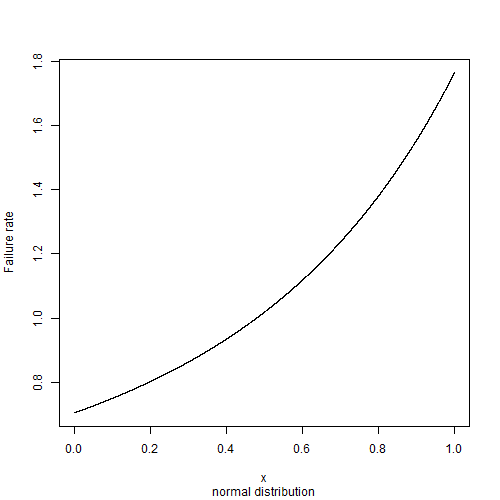
\includegraphics[width=0.8\textwidth]{dnorm.png}
	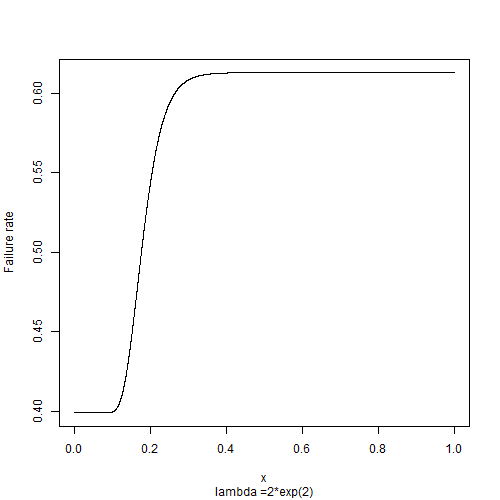
\includegraphics[width=0.8\textwidth]{d2.png}		
\end{minipage}\begin{minipage}[h]{0.5\textwidth}
	\centering
	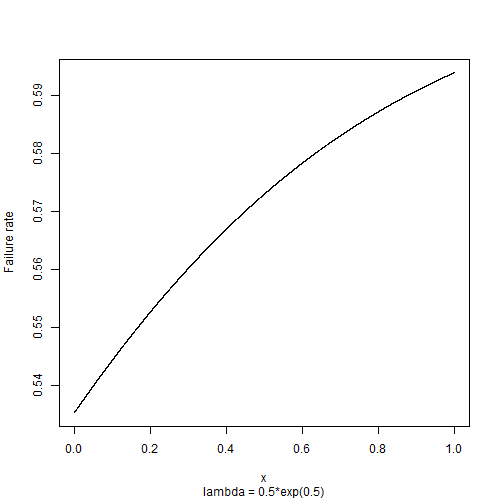
\includegraphics[width=0.8\textwidth]{d05.png} 	
\end{minipage}

\subsection*{e)}
Am letzten Diagramm kann man die Unabhängigkeit von x sehr gut erkennen.
die Failure rate ist im bereich 0.4-1 konstant obwohl sich x ändert.

\section*{Aufgabe 4}

	\subsection*{a)}
	 \begin{center}
	 	Max = 1633 , Min = 0 , Avg = 1026,867
	 \end{center}
	\subsection*{b)}
		\centering
		$P(1200 \leq X \leq 1400) = \frac{\#DaysWithinRange}{\#TotalDays}=\frac{5}{30} = 0.1\overline{6} = 16,\overline{6}\%$ 
		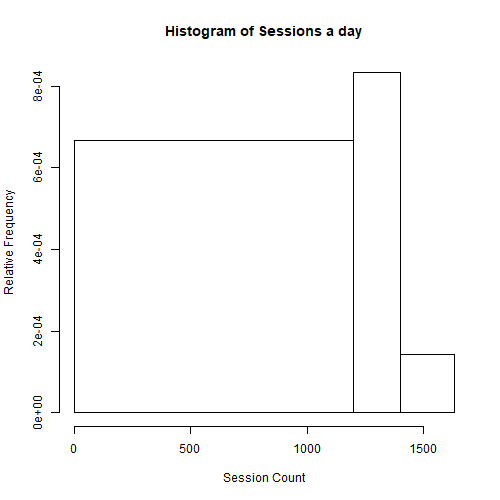
\includegraphics[width=0.5\textwidth]{4histo.png}\\
		Breaks used: 0,1200,1400,163
	\newpage
	\subsection*{c)}
		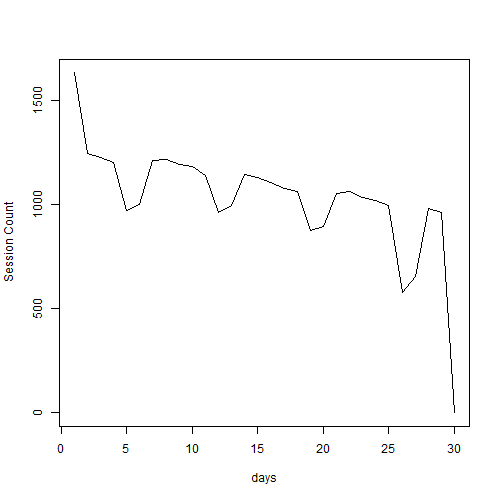
\includegraphics[width=0.5\textwidth]{distr.png}\\
		Am Tag 1 ist die Spitzenlast bereits erreicht.
		Durch das benutzen von zeitlich enger zusammen liegenden Messpunkten würde sich der Zeitpunkt in dem die Spitzenlast genauer bestimmen lassen. Je nachdem wie man die Spitzenlast vorher bestimmt hat könnt sie sinken (durch Verteilung auf kleinere Abschnitte) oder steigen (Registrierung von Sessions, die zwischen den vorherigen Messpunkten lagen.).
		
		
	
	
	
	
	
	
	
	
\end{document}